\section*{Ejercicio 3}
\graphicspath{{Figuras/}}

En este caso se busco implementar una RN para resolver el mapeo logístico dado por la ecuación ${{x(t+1) = 4x(t)(1-x(t))}}$. En este caso la arquitectura de la red puede observarse en la Fig. \ref{03:fig:Arquitectura}, consistiendo en en una capa densa oculta con activación \texttt{sigmoide} y una capa de salida de una neurona con activación lineal. Como función de costo se utilizo MSE. 

Se utilizaron tres valores distintos para la cantidad de datos de entrenamiento, siendo estos 5, 10 y 100. En los tres casos, los datos fueron tomados aleatoriamente con una distribución uniforme entre $0$ y $1$. La red se entreno de manera que realizar una predicción de un dado dato sea equivalente a realizar una iteración en el mapeo logístico. El entrenamiento se realizo durante 1000 épocas. Como conjunto de validación y de test se usaron dos conjuntos de 100 datos con la misma distribución que los datos de entrenamiento. El conjunto de validación se utilizo para seleccionar los hiperparametros, mientras que el de test se utilizo para evaluar la \textit{performance} final de la red luego de concluir el entrenamiento.


%Como datos de entrada se realizo un \texttt{linspace} entre 0 y 1 con 1000000 valores, manteniendo un 10\% de los puntos como validación y otro 10\% como test. A la izquierda en la Figura \ref{fig:5} se observa la evolución de la función de costo en el entrenamiento. 

\begin{figure}[h!]
    \centering
    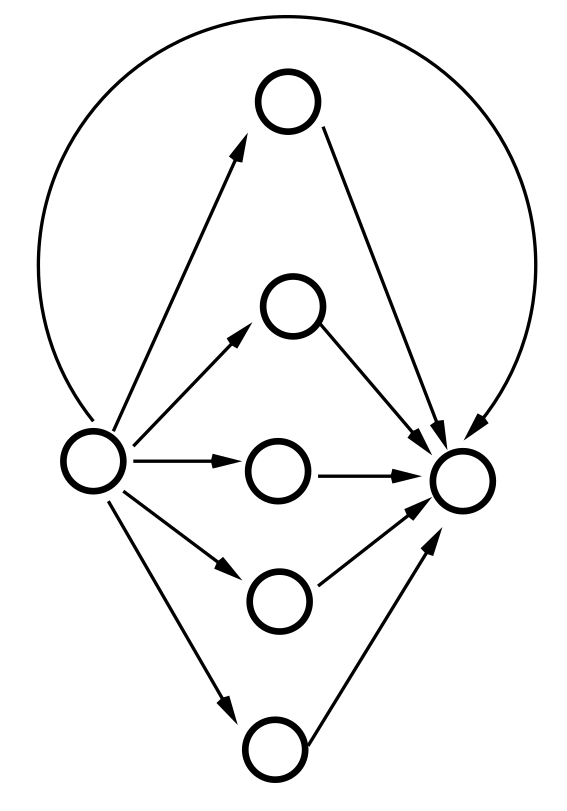
\includegraphics[width=0.3\textwidth]{Figuras/ejer_3.png}
    \caption{Esquema de la arquitectura utilizada para resolver el problema del mapeo logístico.}
    \label{03:fig:Arquitectura}
\end{figure}

En la Fig. \ref{03:fig:Resultados} se observan los resultados obtenidos para la función de costo tanto para los datos de entrenamiento como los de validación, variando la cantidad de ejemplos con los cuales la red es entrenada. Como es de esperarse, la función de costo es menor cuando mayor cantidad de datos de entrenamiento son proporcionados a la red. En todos los casos, el error con los datos de test luego de entrenar fueron cercanos a los valores finales del error con los datos de validación. Cabe destacar que, para la red entrenada con 5 ejemplos, el error con los datos de validación es menor que los obtenidos con los datos de entrenamiento, lo cual no es comportamiento típico, ya que lo usual es que el error de entrenamiento sea menor, ya que es este error el que la red buscara minimizar, independientemente lo que suceda con el error de validación. Sin embargo, la situación no es imposible y puede deberse solo a la poca cantidad de datos presentados para el entrenamiento. 

\begin{figure}[h!]
    \centering
    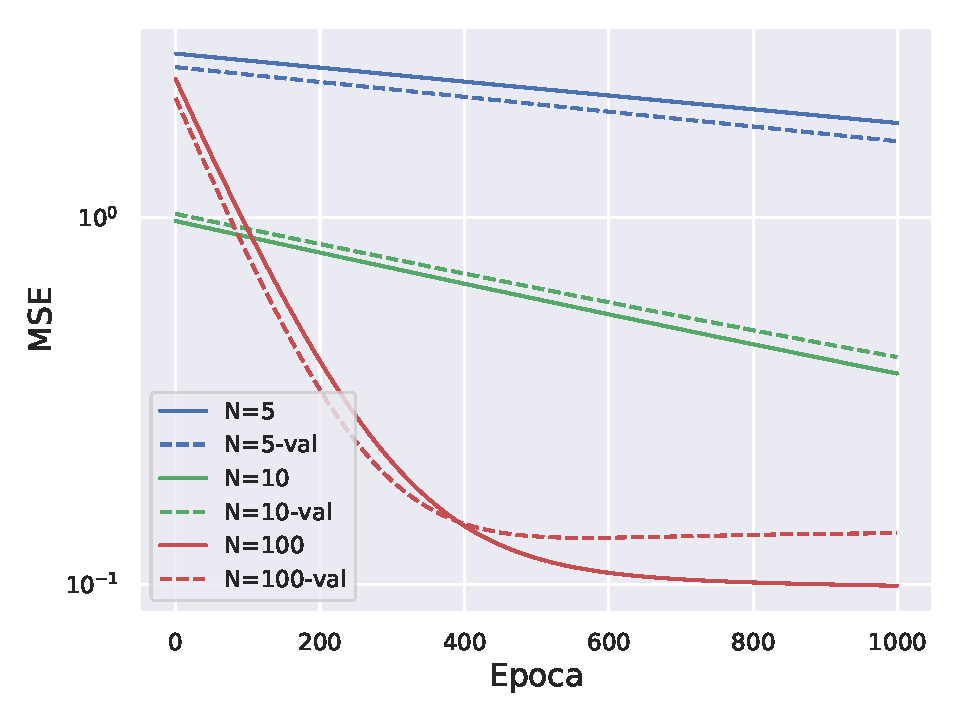
\includegraphics[width=0.75\textwidth]{Figuras/ej3/Loss.pdf}
    \caption{Evolución de la función de costo (presentada en escala logarítmica) tanto para los datos de entrenamiento como los de validación, para los tres modelos entrenados variando la cantidad de ejemplos utilizados para el entrenamiento.}
    \label{03:fig:Resultados}
\end{figure}

Luego, solo para estudiar la utilidad de la red neuronal para estudiar la evolución de un sistema dado por el mapeo logístico, se entreno un nuevo modelo con la misma arquitectura, pero esta vez utilizando 1000000 datos de entrenamiento, equispaciados entre 0 y 1. Como conjuntos de validación y de test se utilizaron dos conjuntos de 500 datos aleatorios entre 0 y 1. A la izquierda en la Fig. \ref{fig:3_Resultados_Largo} se observa la evolución de la función de costo para los datos de validación y de entrenamiento a lo largo de 200 épocas.


\begin{figure}[h!]
    \centering
    \begin{subfigure}[h]{0.49\textwidth} 
        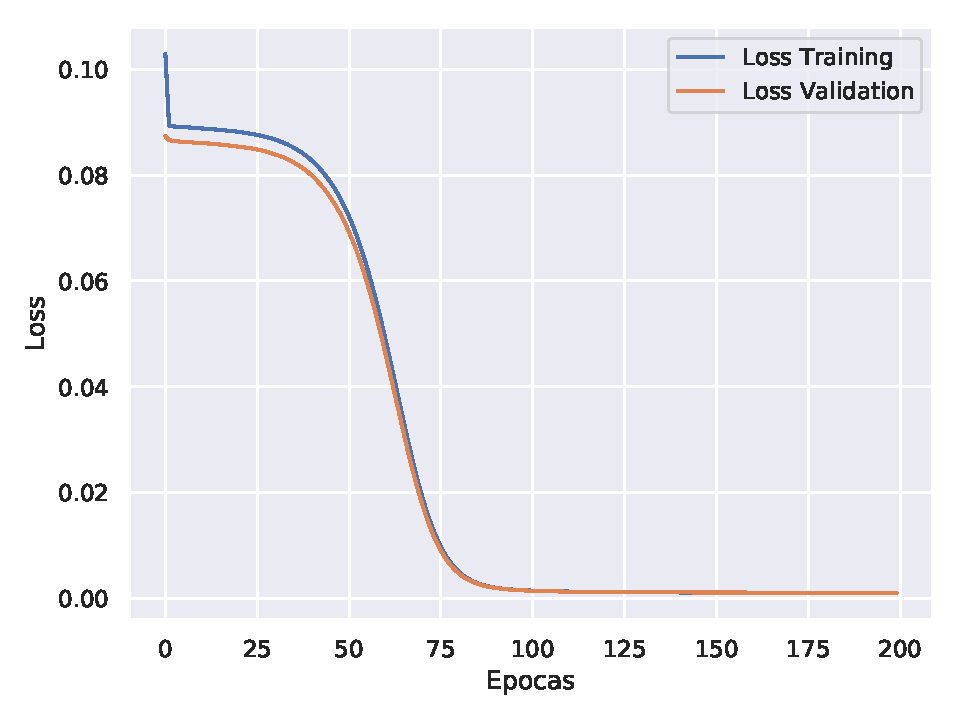
\includegraphics[width=\textwidth]{Figuras/ej3/Largo_Loss.pdf}
    \end{subfigure}       
    \begin{subfigure}[h]{0.49\textwidth} 
        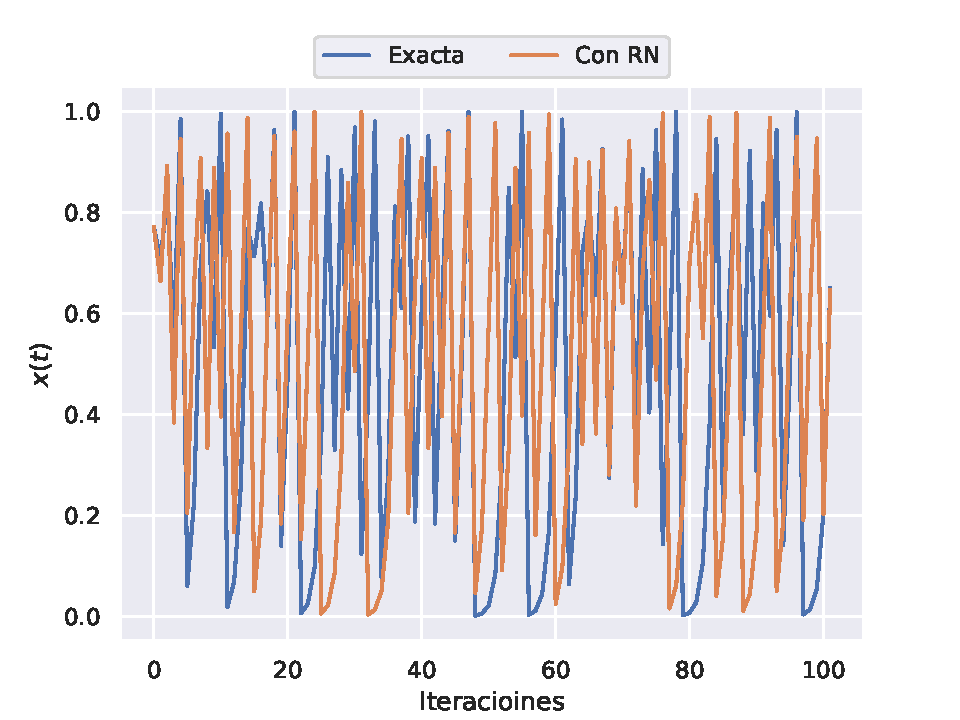
\includegraphics[width=\textwidth]{Figuras/ej3/Largo_Evolucion.pdf}
    \end{subfigure}
    \caption{A la izquierda, se observa la función de costo durante el entrenamiento de la red. Por otro lado, a la derecha, se observa una comparación entre la evolución del mapeo logístico utilizando la red entrenada y utilizando la red exacta. Se observa que la red entrenada no logra reproducir la evolución del sistema.} \label{fig:3_Resultados_Largo}
\end{figure}

Un vez finalizado el entrenamiento de la red, se busco comparar su rendimiento respecto a la evolución exacta. Para esto, se realizaron 100 iteraciones utilizando tanto la red entrenada como la ecuación exacta, con una misma semilla (es decir, un valor de $x(t=0)$) inicializada de manera aleatoria entre 0 y 1. A la derecha de la Figura \ref{fig:3_Resultados_Largo} se observa una comparación de la evolución del problema a partir de ambos métodos. Se observa que el resultado obtenido a partir de la red neuronal no se corresponde con el obtenido de manera exacta, incluso para las primeras iteraciones. Esto se debe al carácter caótico de la del mapeo, en donde una pequeña perturbación de las condiciones iniciales produce un comportamiento notablemente distinto a medida que evoluciona el sistema. Dado que la red entrenada no predice los valores con una precisión absoluta, este error cometido en cada iteración conlleva a evolución significativamente distintas. De este análisis se desprende que el uso de redes neuronales para el estudio de sistemas caóticos puede conllevar a resultados erróneos.